\clearpage
\fancyhf{}
\fancyhead[c]{Chapter 1. General Introduction}% <- added
\fancyfoot[R]{\thepage\ifodd\value{page}\else\hfill\fi}
%\fancyhead[L]{\ifodd\value{page}\relax\else\hfill\fi Ch \thechapter}
%\renewcommand\headrulewidth{0pt}% default ist .4pt
\renewcommand{\plainheadrulewidth}{.4pt}% default is 0pt

\newpage


\noindent I urge you to look around you and observe the trees, the leaves on them, each one with a unique shape and size, isn't it? Look at the people surrounding you, 
how they have different skin colors, facial features, heights, voice and thoughts. Now take a look at your palm, go ahead and examine it. What do you see? Aren't all 
five of your fingers diffent from each other? If you look even closer, you'd see that even the scales and crevices on your fingers are not the same. Have you ever 
wondered why nothing is exactly the same? Variance is an essential feature of nature; it permeates everything, from our thoughts and dreams to our language and societies. 
Without this diversity, life would be sterile, perhaps even impossible.

In this thesis, I have sought to understand the origins and implications of these differences at the most fundamental level: the neurons inside our brains. 
By exploring the variability among these building blocks of thought, ideas, dreams, language, and personality, I aim to shed light on how diversity shapes not only our individual experiences but also the very fabric of life.

\section{Neuronal heterogeneity through the lens of the past}

The mammalian brain is an extraordinarily complex organ, composed of an immense variety of neuronal cell types. This diversity is evident across multiple dimensions, exploring this diversity has been a central tenet in neuroscience, since its inception, dating back to Ramon y Cajal (\cite{fishell2013neuron, huang2019diversity, markram2004interneurons, mukamel2019perspectives, nelson2006problem, petilla2008petilla, sanes2015types, seung2014neuronal, somogyi2005defined, yuste2020community, zeng2022cell, zeng2017neuronal}). I would like to take the reader through what we already know about neuronal heterogeneity via different modalities, ranging from shapes to molecular composition.    

\subsection{Morphology}

Neurons differ dramatically in their shapes and structures. Some, like pyramidal neurons, exhibit long apical dendrites and a characteristic triangular soma, while others, such as inter-neurons, display more compact and intricate branching patterns. These morphological differences are closely linked to the specific roles neurons play within neural circuits (\cite{liu2024neuronal}).


\subsection{Electrophysiology}

Neuronal diversity is also exhibited in the ways neurons generate and propagate electrical signals. Neurons exhibit distinct firing patterns, action potential shapes, adaptation and selectivity to synaptic input. For instance, some neurons are fast-spiking, while others display adapting or bursting firing patterns. These electrophysiological properties are determined by the unique composition of ion channels and receptors expressed by each neuron (\cite{huang2019diversity, markram2004interneurons, mukamel2019perspectives, fishell2013neuron, masland2012neuronal, tasic2018shared, zeng2017neuronal}).


\subsection{Gene Expression}

Advances in molecular biology have revealed that neurons can be distinguished by their gene expression profiles. Single-cell RNA sequencing has enabled researchers to catalog the transcriptomes of individual neurons, uncovering a rich landscape of molecular identities. These profiles often correlate with, but are not strictly determined by, morphological and electrophysiological features (\cite{wagner2016revealing, shapiro2013single, trapnell2015defining}).


\subsection{Connectivity}

Neurons are further defined by their patterns of connectivity, both the sources of their inputs and the targets of their outputs. Some neurons form long-range projections across brain regions, while others participate in local microcircuits. The connectivity matrix of the brain is thus shaped by the diversity of its neuronal components. (\cite{Wang2021, Zhang2024, Gollo2020, Goldman2023, Tripathy2017, Sagner2019} )

\subsection{Patch-seq}
The state of the art in recording neuronal data is a technique known as patch-seq (\cite{cadwell2016electrophysiological, fuzik2016integration}), whereby it is possible to simultaneously record morphological, electrophysiological and molecular properties of neurons. This technique is really powerful as it provides a multi-modal perspective on neuronal heterogeneity. This technique has been the linchpin in some of the biggest classification efforts such by the Allen Brain database (\cite{gouwens2019classification, gouwens2020integrated}).   

\subsection{Large-Scale Taxonomy Initiatives}


In the past decade, large-scale collaborative efforts have sought to systematically map and classify the full diversity of neurons in the brain. Notable among these are the Allen Institute for Brain Science's Cell Types Program and the BRAIN Initiative Cell Census Network (BICCN). These projects leverage cutting-edge techniques, including high-throughput single-cell transcriptomics, large-scale electrophysiological recordings, and high-resolution imaging to build comprehensive taxonomies of neuronal types \cite{gouwens2019classification,gouwens2020integrated}.

While these initiatives have greatly expanded our understanding of neuronal diversity, they often operate under the assumption that neuronal identity is static and can be captured by a fixed set of features. However, emerging evidence suggests that neuronal identity may be more dynamic and context-dependent than previously thought, raising important questions about how best to define and classify the brain's myriad cell types.

\subsection{Traditional Classification Approaches}

Historically, neuroscientists have sought to classify neurons into discrete “types” based on intrinsic, relatively stable characteristics. Early classification schemes focused on observable features such as soma size, dendritic arborization, and axonal projections. With the advent of intracellular recording techniques, electrophysiological properties like spike shape, firing rate, and synaptic integration became central to neuronal taxonomy. More recently, molecular markers such as the expression of specific neurotransmitters, calcium-binding proteins, or transcription factors have been used to further refine neuronal classifications.

The underlying assumption in many of these approaches is that each neuron possesses a fixed identity: a stable set of features that persists across time and context. This has led to the widespread use of terms like “cell type” and “canonical neuron”, suggesting a degree of invariance in neuronal identity.

\section{Limitations of Static Neuronal Classification}

\begin{itemize}
    \item \textbf{The Influence of Input and Network State on Neuronal Function} Recent experimental and computational efforts have increasingly pointed towards the idea that a neuron's functional role is not solely determined by its intrinsic static properties such as morphology, gene expression, or ion channel dynamics but also by the nature of the input it receives and its dynamic state within a circuit \cite{hernath2019alternative,szabo2021conventional}. Neurons operate within continuously changing environments, receiving temporally structured synaptic input that reflects sensory stimuli, behavioral demands, and ongoing internal activity. These inputs interact with intrinsic biophysical parameters in complex ways, such that the same neuron may perform different computational roles depending on the input regime or network context. Additionally, neuromodulatory systems (e.g., dopaminergic and cholinergic pathways) further reconfigure neuronal function in a cell-type- and receptor-specific manner, modulating excitability, gain, adaptation, and stimulus selectivity. This context-dependence challenges the classical view of neurons as fixed computational units. 
    
    \item \textbf{Continuous neuronal identity}
    Recent large scale neuronal classification effort has consistently shown that neurons are not discrete modular classes but rather their electrophysiological, molecular and morphological properties lie on a continuum \cite{marsat2010neural,angelo2012biophysical,scala2021phenotypic}. This further complicates the effort of contextualizing neurons in classes. 

    \item \textbf{Limitations of Static Characterization Protocols} Conventional approaches to neuronal classification typically rely on static stimulation protocols, such as step-and-hold current injections, to derive electrophysiological signatures. While these protocols offer insights into baseline excitability and passive membrane properties, they do not capture the complex temporal filtering or nonlinear input-output transformations that neurons perform under more realistic, time-varying conditions. In naturalistic settings, neuronal input is dynamic, high-dimensional, and often stochastic features that are absent in traditional measurements. As a result, static protocols risk underestimating or mis-characterizing the functional capabilities of neurons, potentially leading to oversimplified or misleading classifications. This disconnect highlights the need for stimulus-rich paradigms, such as frozen noise inputs or in vivo recordings, that better approximate the computational demands faced by neurons in situ.

    \item \textbf{Neuronal Identity as an Emergent, Dynamic Construct} Taken together, these observations point toward a new conceptual framework in which neuronal identity is not a fixed property, but rather a context-sensitive, emergent phenomenon. If neuronal function can be reshaped by synaptic input, neuromodulatory state, and network dynamics, then identity must be understood as fluid and multidimensional, rather than static and categorical. This dynamic view aligns with recent findings showing that neurons shift their classification depending on the input stimulus or modulatory condition. It also suggests that functional heterogeneity in neural populations is not simply biological variability, but may reflect adaptive specialization to a range of computational roles. 

    In this thesis, I explore this emergent view by analyzing how neurons reorganize their functional attributes under different input regimes and neuromodulatory conditions, using high-dimensional clustering and integrative analysis across multiple feature domains. This work contributes to a growing shift in neuroscience: from static taxonomies to dynamic, functionally grounded models of neuronal identity.
    
    \item \textbf{Rich high-dimensional functional space remains unexplored} Neurons functional space is high dimensional but most electrophysiological classification only consider one feature at a time for separability. This leads to an incomplete picture of functional heterogeneity.  As we have discussed before, stimulus protocols have a strong role to play in features that can actually be extracted. For example a static input protocol doesn't expose the subthreshold potential dynamics of a neuron, similar properties related to action potential are a function of input protocol. Clustering based on these features typically involves looking at low dimensional (1-3 dimensions) feature space using a method such as K-means clustering. This approach underestimates the rich functional space in which neurons function and thus clustering based on functional properties needs method that utilize multiple features pertaining to function simultaneously and provide a richer overview of functional heterogeneity. 
    
    \item   \textbf{No consensus on properties that are the most informative about heterogeneity} While neurons have been categorized based active and passive features there is no consensus on properties or a set of properties that are the most informative about heterogeneity. While most classification studies focus on passive properties such as capacitance or conductance of the cell or active properties such as firing rates and inter-spike intervals, there are no studies that compare neuronal heterogeneity based on different sets of properties and provide a consensus for the field. Moreover, the properties extracted are limited by the stimulation protocol, therefore we must first establish the input protocol that is most suitable for studying a neuronal population and then compare properties extracted in each protocol to provide a consensus.  
    

\end{itemize}

\section{Neuromodulation: Reconfiguring Neural Computation}

Neuromodulatory systems particularly those involving dopamine and acetylcholine play a critical role in shaping brain states associated with attention, learning, memory, and pathology. Rather than directly triggering spikes, these modulators reshape how neurons respond to input, modulating intrinsic excitability and synaptic integration. Their effects are often receptor and cell-type-specific, suggesting a finely tuned mechanism for reconfiguring the computational landscape of cortical networks.

Despite extensive behavioral and molecular work, the functional impact of neuromodulation on neuronal computation remains poorly understood, especially at the level of high-dimensional feature interactions. Are neuromodulatory effects isolated to individual electrophysiological features, or do they act in a coordinated manner to restructure how neurons encode information?

\begin{itemize}
    \item \textbf{Effect of neuromodulation on computation} Much is known about molecular and excitability changes caused by dopamine and acetylcholine modulation in single neurons. Though it is still unclear how this alteration changes what neurons compute. Since neurons relay information within a network, it is unclear how dopamine and acetylcholine changes information transfer in neurons. Since activity of individual neurons determine that state of a network, it is clear that understanding alteration in transferred information due to neuromodulation would explain a lot about how cortical circuits are modulated. 

    \item \textbf{Hetero modulation in neuronal population} A given population of neuron comprises of individuals or sub-groups of neurons that differ from each other in terms of their shape and and ion-channel type and distribution. It is still unclear how this individual variability manifests itself on a circuit scale. While it is known that this heterogeneity provides flexibility to  the circuit \cite{wu2025neural,hutt2023intrinsic}, the effect of neuromodulation on this individuality is still unclear. More precisely, it is unknown if all functional parameters are altered uniformly or there exists a heterogeneity in terms of properties that are altered due to specific modulation and what are population level effects of neuromodulation. 

    \item \textbf{Reconfiguration under the influence of dopamine and acetylcholine} Most studies that focus on neuromodulation of individual neurons, focus on how individual active or passive properties such as firing rate or conductance is altered due to a specific receptor activation. Neuronal functional space is high dimensional, while it is important to study how individual properties are altered due to neuromodulation, it is also important to study how this high-dimensional functional space is altered due to neuromodulation, that requires looking at correlation structure between active and passive properties and how this structure changes due to neuromodulation.
\end{itemize}
          
\section{Effect of Temporal Heterogeneity in Artificial Systems}

Biological neural systems are composed of heterogeneous computational units  individual neurons with diverse intrinsic properties \cite{koch1999complexity}. This diversity has been shown to support critical functions such as motor control \cite{cavanagh2020diversity} and memory formation \cite{mcnaughton2006path, hasson2008hierarchical, chu2020long}. While this fact is well-accepted in neuroscience, most artificial neural networks continue to be designed with homogeneous units, particularly in recurrent architectures.

Recurrent Neural Networks (RNNs), which possess temporal memory, have been proposed as functional analogs to biological circuits \cite{sussillo2014neural}. One popular subclass, Reservoir Computing (RC), specifically Echo State Networks (ESNs), has demonstrated the capacity to solve tasks requiring short-term memory \cite{jaeger2001echo}. However, these networks are typically built with uniform time constants and lack the diversity observed in biological systems.

Recent studies have introduced architectural temporal heterogeneity through mechanisms like delay lines in particular, Distance-Dependent Delay Networks (DDNs) which outperform classical ESNs on memory and chaotic time-series tasks \cite{iacob2022distance, soriano2014delay, perez2021neural}. These results suggest that incorporating temporal diversity improves computational performance. However, in such models, heterogeneity is embedded in network-level topology, not in the intrinsic properties of individual units.

Thus, it remains unclear how intrinsic temporal heterogeneity such as variability in decay rates or integration time constants across units influences network performance. This chapter explores this gap by systematically varying internal timescales within reservoir units, testing whether biologically inspired temporal diversity can enhance memory capacity and task performance in artificial networks.


\section{Research Objectives and Key Questions}
This thesis addresses two overarching questions:
\begin{enumerate}
  \item \textbf{How does input context influence functional classification of neurons?} \\
  In Chapter 2, we demonstrate that neuronal identity is not static, but input-dependent, with classification outcomes varying significantly under dynamic (frozen noise) vs static (step-and-hold) stimuli. This challenges the notion of fixed electrophysiological types and highlights the role of stimulus structure in shaping neural function.

  \item \textbf{How does neuromodulation alter the functional landscape of neurons?} \\
  In Chapter 3, we explore how activation of dopaminergic (D1-R, D2-R) and cholinergic (M1-R) receptors reconfigures information encoding, shifting the balance between shared and private variance across feature domains. We show that neuromodulatory effects are highly cell-type and receptor-specific, modulating not just individual attributes but also their coordination.

  \item \textbf{Can intrinsic timescale heterogeneity improve performance and memory in reservoir computing systems?} \\
  In Chapter 4, we design 4 different variants of ESNs and DDNs with varying levels of timescale heterogeneity and optimize them to perform NARMA-30 and Mackey-Glass benchmark tasks. We study the effect of the designed heterogeneity on task performance, stability, representation and memory capacity. We show that an intermediate level of heterogeneity is optimum for solving the two benchmark tasks, suggesting heterogeneity requirement is task dependent.     
  
\end{enumerate}


\section{Experimental Framework and Approach}

For answering the research questions stated above, this thesis utilizes single unit in-vitro recordings form the somatosensory cortex layer 2/3 \cite{da2018databank}. These recordings were performed in tandem, first using a static step and hold input protocol and later with a frozen noise protocol. Within each input protocol, neurons were first recorded in a vehicle control (artificial cerebral spinal fluid - aCSF) condition and a drug condition, where a specific receptor agonist is added to the bath and the recording is performed again. Some times multiple control and drug trials are performed for a single neuron.   

\subsection{Input Protocols }
\begin{figure}
    \centering
    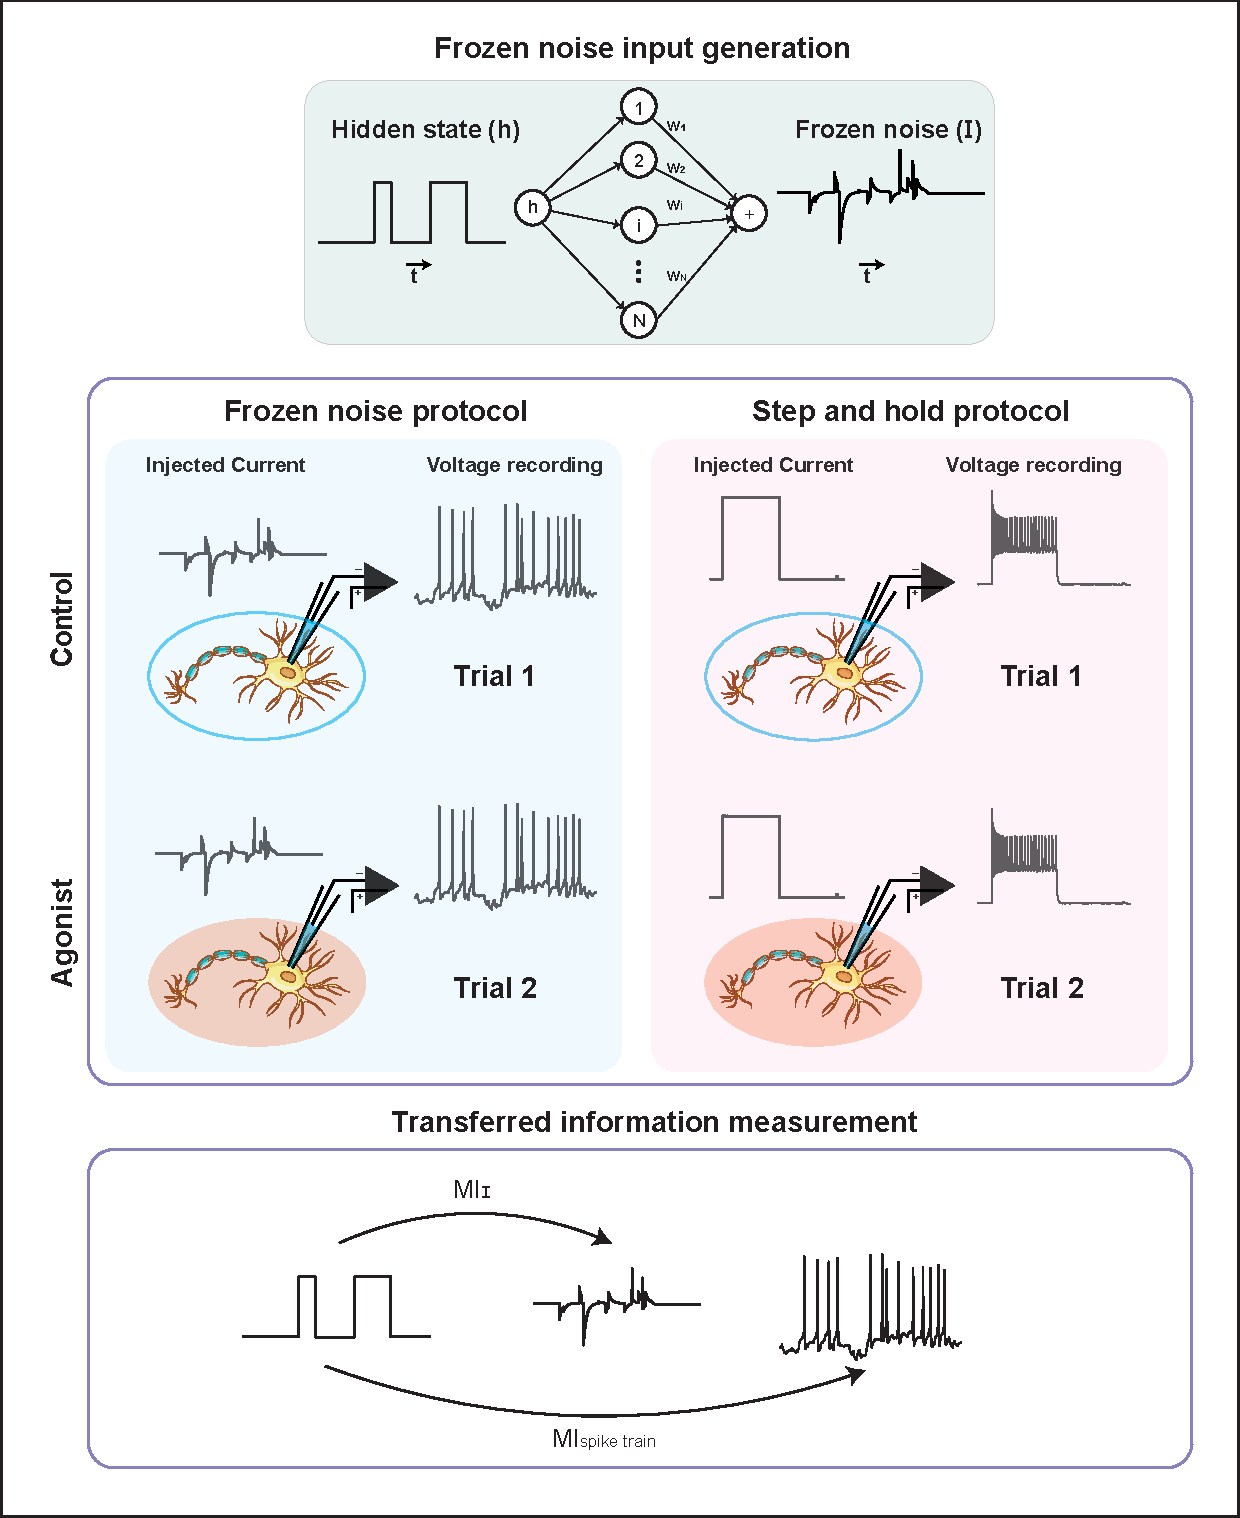
\includegraphics[width=\linewidth]{Figures/Intro/input_protocol.pdf}
    \caption{\textbf{Data collection and input protocol}}
    \label{fig:enter-label}
\end{figure}
\subsubsection{Step and Hold }
The step-and-hold protocol is a widely used electrophysiological method for characterizing neuronal properties through controlled current injections. In this protocol, a neuron's membrane potential is maintained at a baseline value (commonly around -70 mV), and then a series of incremental current steps are injected, each lasting for a fixed duration, typically 500 ms with recovery periods (e.g., 5.5 seconds) between steps. The current amplitude is increased in defined increments (e.g., 40 pA per step), allowing researchers to observe how the neuron responds to increasing levels of depolarizing input, including changes in firing rate, spike threshold, and other action potential characteristics. This approach enables the classification of neurons (such as distinguishing excitatory from inhibitory cells) and the assessment of properties like maximum firing frequency, spike latency, and after-hyperpolarization. The step-and-hold protocol thus provides a standardized way to probe intrinsic excitability and firing dynamics, serving as a foundational tool in cellular neurophysiology. 
\subsubsection{Frozen Noise }
The frozen noise protocol \cite{zeldenrust2017estimating}, is a method designed to quantify the mutual information between a neuron's input and its spike train output in electrophysiological experiments. This protocol generates a time-varying input current by simulating the activity of a presynaptic neural network of 1,000 neurons, each firing Poisson spike trains in response to a binary "hidden state" (a Markov process representing the presence or absence of an external stimulus). The injected current is "frozen," meaning the same input sequence is used across trials or conditions, enabling direct comparison of neuronal responses. By analyzing how the recorded neuron transforms this structured input into spikes, researchers can calculate the information-theoretic relationship between the hidden state and the output spike train. This approach overcomes limitations of traditional step-and-hold protocols by mimicking naturalistic synaptic input patterns while maintaining experimental control, allowing efficient bias-free information quantification with short (6 minute) recordings. The protocol's output includes the injected current trace, hidden state timeline, and voltage response, facilitating both forward modeling of neuronal dynamics and reverse-engineering of coding principles. 

\subsection{Extracted features}
We analyze neuronal function across four distinct attribute sets:
\begin{itemize}
  \item \textbf{Action Potential (AP) Dynamics}
  \item \textbf{Passive Biophysical (PB) attributes}
  \item \textbf{Adaptation Currents (AC)} 
  \item \textbf{Input Feature Selectivity}, estimated using \textbf{Spike-Triggered Averages (STA)}
\end{itemize}

To dissect the specificity and dynamics of neuronal encoding depending on input and neuromodulation, we apply unsupervised high-dimensional clustering \cite{lee2021non}, cosine similarity analysis, and Mult-iset Correlation and Factor Analysis (MCFA) \cite{brown2023multiset}. These methods allow us to examine both within-domain variance and cross-domain coordination of features, offering a system-level view of functional reconfiguration.
\begin{figure}
    \centering
    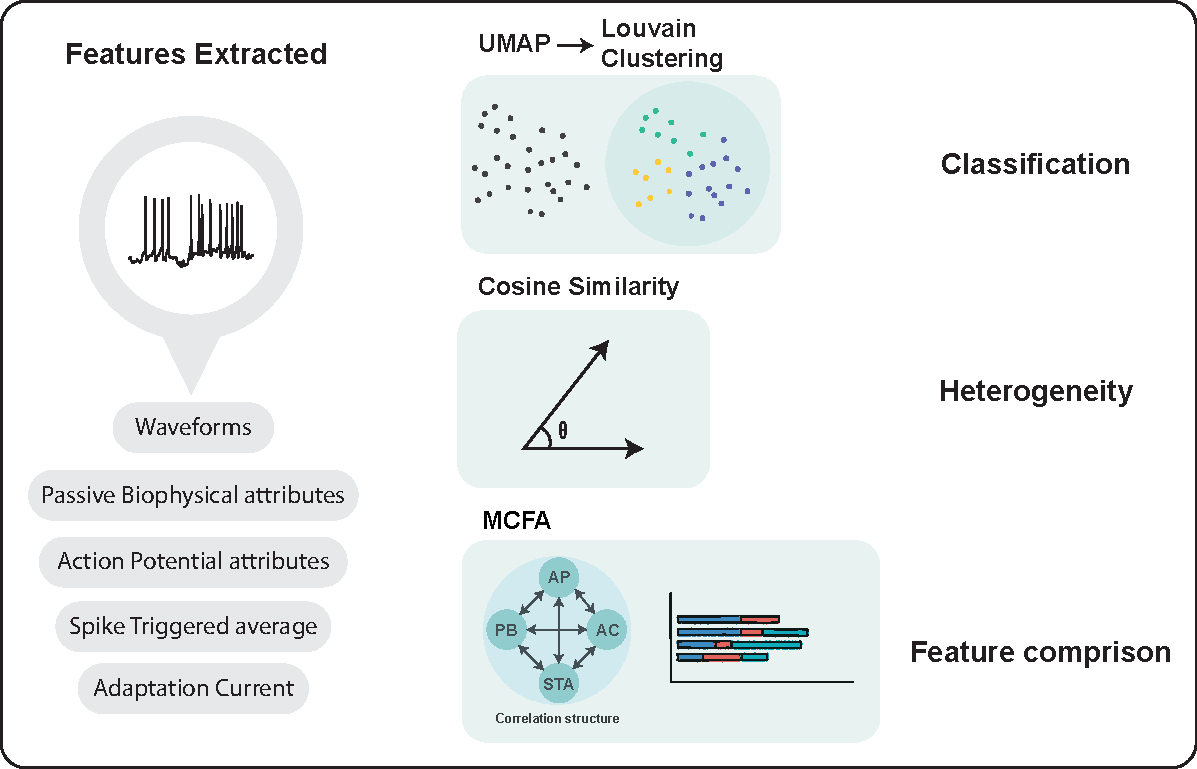
\includegraphics[width=\linewidth]{Figures/Intro/analysis_tools.pdf}
    \caption{\textbf{Overview of extracted features and analysis tools}}
    \label{fig:enter-label}
\end{figure}

\subsection{Network Design}

We designed four different heterogeneity types for ESNs and DDNs: 
\begin{enumerate}
    \item \textbf{Homogeneous Network}: All units share a single decay parameter.
    \item \textbf{Homogeneous Cluster}: The reservoir is divided into clusters, each with its own fixed decay parameter.
    \item \textbf{Heterogeneous Network}: Each unit samples its decay from a shared distribution.
    \item \textbf{Heterogeneous Cluster}: Each cluster samples decay parameters from different distributions.
\end{enumerate}

We tested these networks on two benchmark tasks namely NARMA-30 and Mackey-Glass tasks:
\begin{itemize}
    \item \textbf{NARMA-30}: A nonlinear auto-regressive moving average task designed to test long-range memory and nonlinear dynamics. 
    \item \textbf{Mackey-Glass}: A chaotic time-series prediction task that evaluates a network's ability to generate stable yet complex temporal outputs.
\end{itemize} 


\section{Summary and Outlook}

This introduction has outlined the motivation and rationale for investigating neuronal identity and function through the dual lenses of input-dependence and neuromodulatory flexibility. Traditional classification approaches, though informative, fall short in capturing the high-dimensional, dynamic nature of neuronal computation. By leveraging frozen noise protocols, multivariate electrophysiological features, and modern unsupervised analysis techniques, this thesis proposes a data-driven framework to redefine neuronal identity as an emergent, context-sensitive construct. Finally, this thesis investigates the computational implications of intrinsic heterogeneity by modeling structured diversity in artificial reservoir systems. The following chapters present experimental results and theoretical insights that collectively support this paradigm shift.

\section{Thesis Structure}
\begin{itemize}
  \item \textbf{Chapter 2}: Neuronal Identity is Not Static: An Input-Driven Perspective \\
  Demonstrates how different stimulation protocols yield distinct classifications, showing that neuronal identity is dynamic and shaped by input.

  \item \textbf{Chapter 3}: Neuromodulatory Control of Cortical Function \\
  Examines how neuromodulators reshape the computational roles of neurons, altering both encoding capacity and feature interdependence.

  \item \textbf{Chapter 4}: Timescale heterogeneity in reservoir computing \\   
    Analyzes the effect of timescale heterogeneity on task performance of ESNs and DDNS, showing that moderate timescale heterogeneity improves the performance over networks without it.  

  \item \textbf{Chapter 5}: General Discussion and Future Directions \\
  Integrates findings across studies, discusses implications for neuroscience and artificial neural networks, and proposes directions for future research.
\end{itemize}





\newpage
\begin{spacing}{1.0} % Set the line spacing to single spacing
\fontsize{8pt}{8pt}\selectfont
\bibliographystyle{apalike}
\renewcommand{\bibname}{References}
\bibliography{All_bibtex}
\end{spacing}